\documentclass{proc}
\usepackage[utf8]{inputenc}
\usepackage{cmap}					% поиск в PDF
\usepackage[T2A]{fontenc}			% кодировка
\usepackage[utf8]{inputenc}			% кодировка исходного текста
\usepackage[english,russian]{babel}	% локализация и переносы
\usepackage{amsmath}
\usepackage{graphicx}
\usepackage{ulem}
\usepackage{soul}
\graphicspath{ {images/} }
\begin{document}
	
	\noindent {\Large \bf Вопросы на ''до свидания''}
	\begin{enumerate}
		
		\item \uline{Полнота, точность}
		
		Полнота, она же Recall - сколько фрода мы поймали.
		
		Точность, Precision - сколько не-фрода мы пропустили.
		
		$$Recall = \frac{tp}{tp+fn}$$
		
		$$Precision = \frac{tp}{tp+fp}$$
		
		\item \uline{ROC кривая. Коэфициент Джини.  AUC}
		
		ROC кривая - зависимость true positive от false positive для разных порогов решающего правила.
		
		Коэффициент Джини - максимальное отклонение ROC кривой от диагонали $tp = fp$.
		
		Если система адекватная (не контрпродуктивная), то кривая всегда будет выше диагонали.
		
		AUC - ''area under curve'' - площадь под кривой ROC. Чем выше, тем лучше.
		
		\item \uline{tp, fp, tn, fn}
		
		\begin{center}
			\begin{tabular}{| c | c | c |}
				\hline
				... & Фрод & Не фрод \\ \hline
				Думаем, что фрод & tp & fp \\ \hline
				Думаем, что не фрод & fn & tn \\ \hline
			\end{tabular}
			
			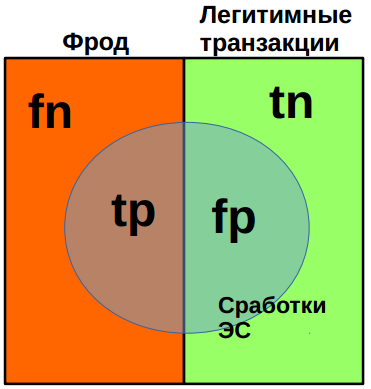
\includegraphics[width=3cm]{tptnfpfn}
		\end{center}
		
		
		\item \uline{классификация}
		
		Есть несколько категорий (напр. фрод$\backslash$не фрод). Необходимо объекты расфасовать по категориям. В ''обучающей выборке'' заранее известно, в какую категорию какой объект входит. 
		
		\item \uline{кластеризация}
		
		Категории заранее неизвестны. Необходимо разбить объекты на несколько ''каких-то'' категорий.
		
		\item \uline{регрессия}
		
		Зная значение функции на каком-то наборе точек, наиболее хорошо приблизить функцию.
		
		\item \uline{идентификация}
		
		Определить, к какой из большого числа категорий принадлежит объект.
		
		\item \uline{обучение с учителем и обучение без учителя}
		
		Supervised$\backslash$Unsupervised learning. При обучении с учителем системе дается какая-то обучающая выборка, для которой задача уже решена (например, при задаче классификации). Без учителя обучающей выборки нет, система сама должна искать закономерности (кластеризация).
		
		\item \uline{признак}
		
		Строго заданная характеристика объекта (например, сумма транзакции в рублях).
		
		\item \uline{класс}
		
		Одна из категорий, принадлежность к которой необходимо определить при решении задачи классификации.
		
		\item \uline{событие, действие, решение}
		
		???
		
		\item \uline{обратная связь}
		
		В общем случае: влияние выхода системы на ее дальнейший вход.
		
		\item \uline{DENY, REVIEW, ALLOW решения ФМ системы RSA}
		
		DENY - заблокировать транзакцию и профиль клиента.
		
		REVIEW - потребовать подтверждение в КЦ.
		
		ALLOW - разрешить без вопросов.
		
		\item \uline{примеры применения машинного обучения для задач информационной безопасности}
		
		Имея транзакции банка, определить фрод.
		
		Зная поведение ботнетов, предсказывать будущие атаки или определять, является ли компьютер частью ботнета.
		
		\item \uline{экспертная система}
		
		???
		
		\item \uline{выброс}
		
		Нестандартные данные, которые могут помешать классификации.
		
		\item \uline{аномалия}
		
		???
		
		\item \uline{выборка}
		
		Конечный набор объектов, взятый из множества всех возможных объектов.
		
		\item \uline{разделяющая гиперповерхность}
		
		Гиперплоскость в пространстве всех возможных объектов, которая разделяет объекты на классы.
		
		\item \uline{функция штрафа}
		
		Некая функция, символизирующая, насколько ''плохо'' был классифицирован объект. Обычно функция расстояния или просто +1 за каждую точку не в своем классе. Задача классификации сводится к задаче минимизации функции штрафа.
		
		\item \uline{логистическая функция}
		
		$$f(\pm d(x_1,x_2))=f(d)=\frac{1}{1-e^{-\alpha \times d}}$$
		
		Используется в качестве функции штрафа.
		
		\item \uline{ансамбль}
		
		Мнения нескольких систем так или иначе аггрегируются в одно (например, функцией голосования).
		
		\item \uline{дерево решений}
		
		Дерево, в каждом узле которого находится условие, определяющее, к какому из детей надо перейти. В листьях содержатся классы. Каждый объект спускается по дереву в соответствии с условиями, пока не попадет в класс.
		
		\item \uline{бутстрепинг}
		
		Генерация выборки размера $N$ из подвыборки размера $n \ll N$ путем выбора с повторением.
		
		\item \uline{бутстреп аггрегация}
		
		Она же bagging. Тот же ансамбль на классификаторах.
		
		Обобщение одного и того же классификатора на различных подвыборках или случайных параметрах, которые различны при каждой новой подгонки.
		
		\item \uline{подгонка (fitting)}
		
		Настройка параметров классификатора с помощью обучающих выборок.
		
		\item \uline{проверка (scoring)}
		
		Оценка качества классификатора на тестовой выборке.
		
		\item \uline{переобучение (overfitting)}
		
		Явление, когда модель слишком точно подогнана под обучающие данные, видя закономерности в случайном шуме. Такая модель может работать хуже на больших данных.
		
		\item \uline{пакеты pandas, numpy, scikit-learn, matplotlib}
		
		Библиотеки для Python.
		
		Pandas - структуры данных.
		
		numpy - матрицы, математика.
		
		scikit-learn - машинное обучение
		
		matplotlib - графики
	\end{enumerate}
	
	\noindent {\Large \bf Вопросы 1}
	\begin{enumerate}
		
		\item 111
		
		
	\end{enumerate}
	
	
	\noindent {\Large \bf Вопросы 2 и 3}
	\begin{enumerate}
		
		
		\item \uline{Задачи классификации, кластеризации и регрессиии.}
		
		Классификация:
		
		Есть набор объектов, каждый из которых принадлежит к какому-то заранее определенному классу. Системе на вход поступает обучающая выборка: набор объектов, для которых класс заведомо известен. Система должна новые поступающие объекты распределять по классам.
		
		Кластеризация:
		
		Есть набор объектов. Необходимо их разбить на какое-то количество кластеров, так что в одном кластере объекты "похожи" друг на друга, а между классами различаются.
		
		Регрессия:
		
		Известно значение функции в точках. Найти функцию.
		
		\item \uline{Задачи регрессии, интерполяции, аппроксимации. Прогнозирование.}
		
		Регрессия:
		
		Известно значение функции в точках. Найти функцию.
		
		Интерполяция:
		
		Известно значение функции в точках. Найти значение в промежуточных точках.
		
		Аппроксимация:
		
		Известно значение функции в точках. Найти приближенное значение функции в других точках.
		
		\sout{Пророчество} Прогнозирование - попытка узнать значение какого-то показателя в будущем, зная, как он вел себя в прошлом.
		
		\item \uline{Задачи ML и DM в информационной безопасности: банковский фрод; pay per click. Суть проблемы и общий подход к решению.}
		
		Задача: среди огромного количества происходящих транзакций выявлять мошеннические и отвергать$\backslash$валидировать подозрительные.
		
		Задача: среди кликов на рекламные баннеры выявлять те, которые реально принесли рекламную пользу (а не являются ботами, например). Начислять деньги только за осмысленные клики.
		
		Решается задача классификации с двумя классами: фрод$\backslash$не фрод или зачислять$\backslash$не зачислять.
		
		\item \uline{Задачи ML и DM в информационной безопасности: call фрод, обнаружение социальной инженерии. Суть проблемы и общий подход к решению.}
		
		???
		
		\item \uline{Задачи ML и DM в информационной безопасности: поведенческий анализ botnet-ов, обнаружение фазинга. Суть проблемы и общий подход к решению.}
		
		???
		
		\item \uline{Полнота и точность. F-мера. Другие метрики оценки качества классификаторов.}
		
		
		
		Полнота, она же Recall - сколько фрода мы поймали.
		
		Точность, Precision - сколько не-фрода мы пропустили.
		
		$$Recall = \frac{tp}{tp+fn}$$
		
		$$Precision = \frac{tp}{tp+fp}$$
		
		F-мера - единый критерий, зависящий от полноты и точности.
		
		$$F_\beta = \frac{(1+\beta^2) \times precision \times recall}{\beta^2 \times precision + recall}$$
		
		Другие метрики:
		
		ROC-кривая, коэффициент Джини. Accuracy ($\frac{tp+tf}{tp+tn+fp+fn}$). Cost-benefit analysis. Value at risk.
		
		
		\item \uline{Расстояние Евклида, манхеттенское расстояние. Расстояние Минковского. Расстояние Чебышева. Расстояние Махаланобиса.}
		
		Расстояние Евклида: $\sqrt{\Delta x^2 + \Delta y^2 + ...}$
		
		Манхэттенское расстояние: $\Delta x + \Delta y + ...$
		
		Расстояние Минковского: $P(x,y)=(\sum_{i=1}^{n}|x_i-y_i|^p)^\frac{1}{p}$
		
		Расстояние Махаланобиса: $d(x_1,x_2)=\sqrt{(x_1-x_2)^T \Delta^{-1} (x_1-x_2)}$, где $\Delta$ - матрица ковариации. Вырождается в евклидово для единичной матрицы ковариации.
		
		\item \uline{ROC кривая. Коэфициент Джини. AUC.}
		
		ROC кривая - зависимость true positive от false positive для разных порогов решающего правила.
		
		Коэффициент Джини - максимальное отклонение ROC кривой от диагонали $tp = fp$.
		
		Если система адекватная (не контрпродуктивная), то кривая всегда будет выше диагонали.
		
		AUC - ''area under curve'' - площадь под кривой ROC. Чем выше, тем лучше.
		
		\item \uline{SSI. VaR, CBA}
		
		System Stability Index: задается отношение двух величин на момент времени $t:x$ и $y=f(x,t)$. Выбираются значения $x_i: \{x_1, x_2, ... x_n\}.$
		
		$$ SSI(t_1,t_2) = \sum_{i=1..n}^{} (f(x_i;t_1)-f(x_i;t_2)) * \log_q \Big(\frac{f(x_i;t_1)}{f(x_i;t_2)}\Big)$$
		
		Cost-Benefit Analysis: оцениваем свойства системы в условных единицах. Определяются затраты того или иного поведения системы. Решается СЛАУ, максимизирующая получаемые единицы.
		
		Value at risk: определяются риски и их ущерб, составляется СЛАУ, минимизирующая этот ущерб.
		
		\item \uline{Признаки, характеристики, контрибьютеры. Сравнимые и несравнимые признаки. Сложные и простые. Непрерывные, дискретные, бинарные.}
		
		Харакеристика --- некое обобщенное свойство предмета.
		
		Признак --- конкретно математически заданное свойство предмета.
		
		Контрибьютор --- совокупность признаков (возможно один), вносящих определенный вклад в априорную вероятность определения класса.
		
		Сравнимые признаки --- те, на пространстве которых можно осмысленно задать полный порядок (например, возраст).
		
		Несравнимые --- для которых никакой порядок не имеет смысла (например, город).
		
		Сложные --- некая композиция простых признаков (например, дата состоит из года, месяца...)
		
		Непрерывные$\backslash$дискретные --- день, когда я не смогу назвать разницу между непрерывным и дискретным без шпаргалки будет днем, когда я уйду на пенсию.
		
		Бинарные --- 2 возможных значения.
		
		\item \uline{Пакеты Python. NumPy, SciPy, Pandas, Matplotlib. Jupyther.}
		
		Pandas --- структуры данных.
		
		numpy --- матрицы, математика.
		
		scikit-learn --- машинное обучение.
		
		matplotlib --- графики.
		
		Jupyter --- web-приложение для создания интерактивных книг с кодом.
		
		\item \uline{Функция штрафа.}
		
		Некая функция, символизирующая, насколько ''плохо'' был классифицирован объект. Обычно функция расстояния или просто +1 за каждую точку не в своем классе. Задача классификации сводится к задаче минимизации функции штрафа.
		
		\item \uline{Байесовский подход. Преимущества и недостатки. Разбиновка. Преимущества и недостатки}
		
		Байесовский подход: имеем априорную вероятность попадания объекта в тот или иной класс. Вычисляем или задаем вероятность, что объект будет иметь определенный набор признаков (отношение правдоподобия). Кладем в теорему байеса, перемешиваем ==> proft.
		
		Наиболее математически ''корректный'', но отношения правдоподобия надо откуда-то взять.
		
		Разбиновка: разбиваем пространство на прямоугольные области. Каждую из областей помечаем каким-то классом. Новые объекты кладем в тот класс, в чей бин он попал.
		
		Крайне легкий в вычислении и реализации, но ограничен в том, какие именно зависимости он может поймать.
		
		\item \uline{Дерево решений. Лес. Случайный лес. Построение случайного леса. Критерии остановки. «Эмпирическая теорема» о случайном лесе.}
		
		Дерево решений --- дерево, в каждом узле которого находится условие, определяющее, к какому из детей надо перейти. В листьях содержатся классы. Каждый объект спускается по дереву в соответствии с условиями, пока не попадет в класс.
		
		Лес --- ансамбль деревьев.
		
		Случайный лес --- лес, построенный случайным образом.
		
		Построение --- случайным образом строится разбиновка. Останавливаемся, если в бине мало элементов, если дерево слишком глубокое или если коэффициент Джини мал. Проверяется ее качество. Если достаточно --- кладем в лес. Повторяем до готовности.
		
		''Эмпирическая теорема'' --- случайный лес хоть как-то работает, если вы не можете придумать ничего лучше.
		
	\end{enumerate}
\end{document}
